%% Standard start of a latex document
\documentclass[letterpaper,12pt]{article}
%% Always use 12pt - it is much easier to read
% \usepackage{algorithm}
% \usepackage{algpseudocode}
\usepackage{float}
\usepackage{xcolor}

%% AMS mathematics packages - they contain many useful fonts and symbols.
\usepackage{amsmath, amsfonts, amssymb}
\usepackage{graphicx}
\usepackage[linesnumbered, ruled, vlined]{algorithm2e}
\usepackage{amsmath}

%% The geometry package changes the margins to use more of the page, I suggest
%% using it because standard latex margins are chosen for articles and letters,
%% not homework.
\usepackage[paper=letterpaper,left=25mm,right=25mm,top=3cm,bottom=25mm]{geometry}
%% For details of how this package work, google the ``latex geometry documentation''.
\usepackage{geometry}
\geometry{
  left=0.5in,
  right=0.5in,
  top=0.8in,
  bottom=1in
}
\usepackage{enumerate}
%%
%% Fancy headers and footers - make the document look nice
\usepackage{fancyhdr} %% for details on how this work, search-engine ``fancyhdr documentation''
% \pagestyle{fancy}
%%
%% This is a little more complicated because we have used `` \\ '' to force a line-break between the name and number.
%%
\newcommand{\Z}{\mathbb{Z}}
\newcommand{\bigO}{\mathcal{O}}

\cfoot{Page \thepage} % page in middle

%% These put horizontal lines between the main text and header and footer.
\renewcommand{\footrulewidth}{0.4pt}
%%%

%%%%%%
%% We shouldnt have to change the stuff above, but if you want to add some newcommands and things like that, then putting them between here and the ``\begin{document}'' is a good idea.
%%%%%%


\begin{document}
% Homework 0 does not contain any mathematics --- it is just for you to practice using latex. All I want you to do is to try to reproduce this document as well as you can. You do not have to hand it in. I don't mind if you work in small groups, but just copying it directly from a friend isn't going to help you later in the term.

\begin{center}
    {\Huge \textbf{Examples}} \\
    Richard Adhika
\end{center}

\

In this file, we run through some examples 
for ratio 1, 2, 3, and 4 (the code can be found in the following files:
'ratio1\_and\_ratio.ipynb', 'ratio3.ipynb', and 'ratio4.ipynb'). 
For outputs of ratio 2, the array represents increasing $kbig$ as specified in each example.
For outputs of ratio 3 and ratio 4, the array represents increasing $e = 0, 1, \dots$.
The following runtime may be inaccurate as (for some unknown reason),
running Julia in WSL (Windows Subsystem for Linux) can cause inconsistent runtime 
(as much as a factor of 2!).
The examples are as follows,
\begin{enumerate}
\item $p=2, n=9, M' = \begin{pmatrix}
1 & 0 \\ 0 & 3
\end{pmatrix}.$ \\
For $kbig = 10, \dots, 17$, $e = 0, \dots, 5$, and $k=n$ for ratio 3, we get \\
\fbox{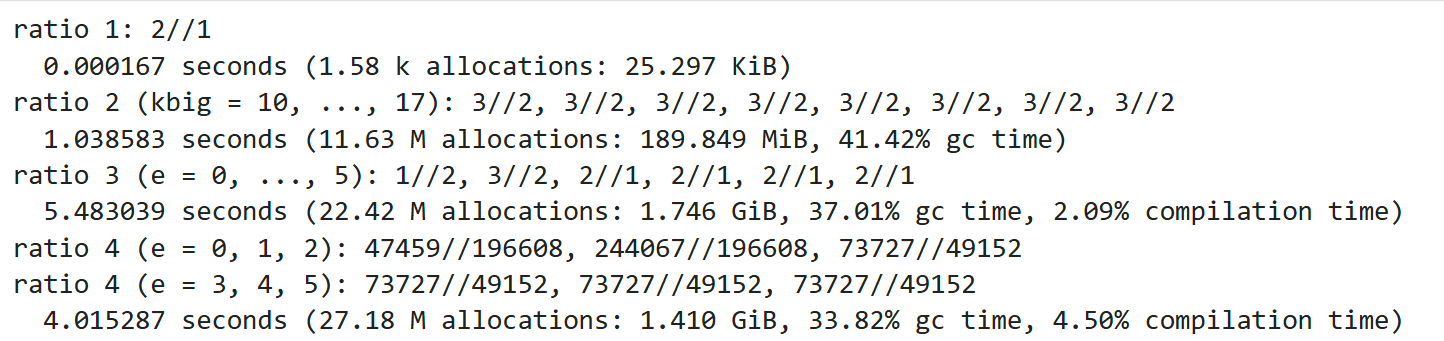
\includegraphics[scale = 0.5]{p2_1.png}} \\

\item $p=2, n=11, M' = \begin{pmatrix}
1 & 0 \\ 0 & 5
\end{pmatrix}.$ \\
For $kbig = 12, \dots, 17$, $e = 0, \dots, 6$, and $k=n$ for ratio 3, we get \\
\fbox{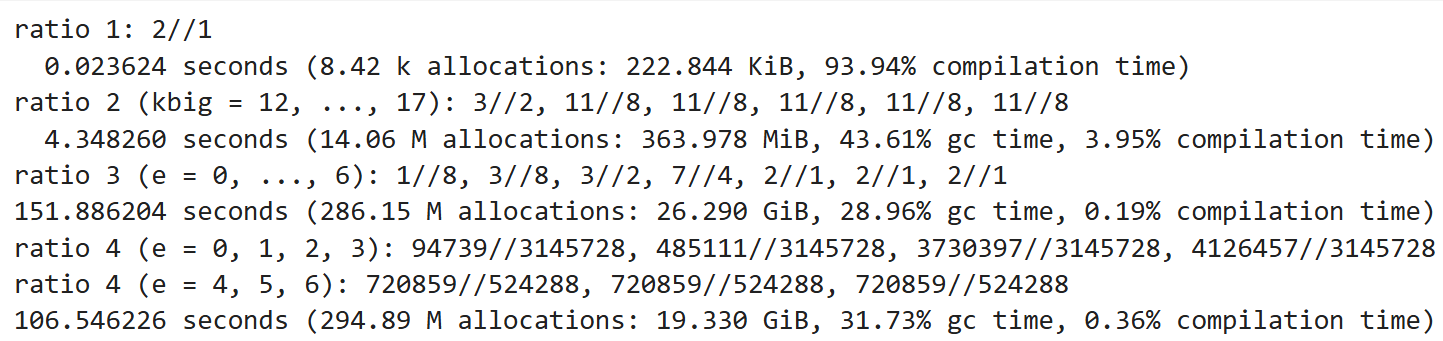
\includegraphics[scale = 0.5]{p2_2.png}} \\

\item $p=2, n=11, M' = \begin{pmatrix}
1 & 0 \\ 0 & 9
\end{pmatrix}.$ \\
For $kbig = 12, \dots, 17$, $e = 0, \dots, 7$ and $k=n$ for ratio 3, we get \\
\fbox{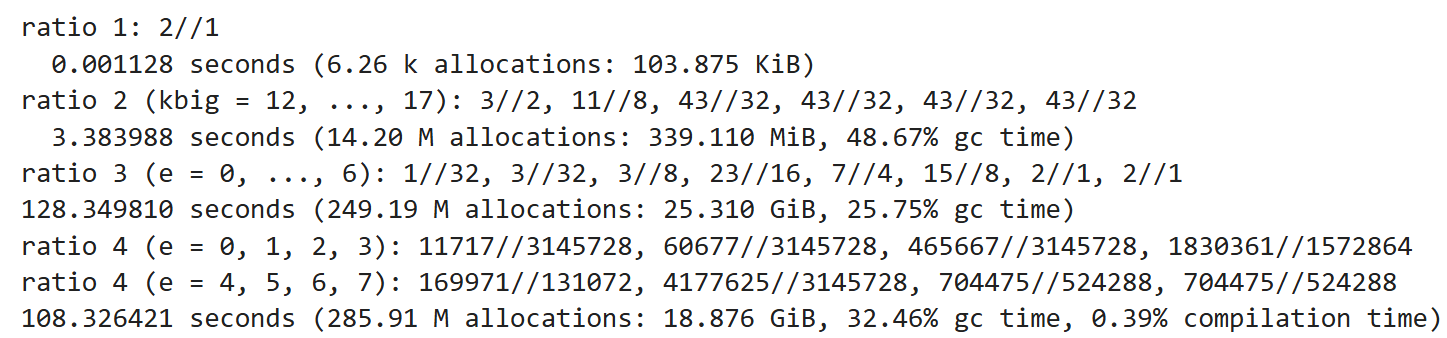
\includegraphics[scale = 0.5]{p2_3.png}} \\

\item $p=3, n=6, M' = \begin{pmatrix}
1 & 0 \\ 0 & 4
\end{pmatrix}.$ \\
For $kbig = 7, \dots, 12$, $e = 0, \dots, 6$ and $k=n$ for ratio 3, we get \\
\fbox{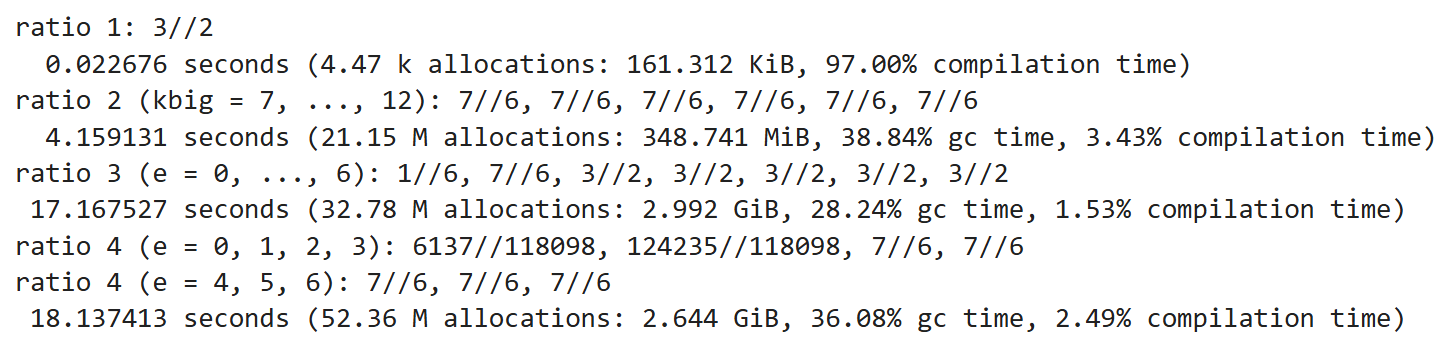
\includegraphics[scale = 0.5]{p3_1.png}} \\

\item $p=3, n=7, M' = \begin{pmatrix}
1 & 0 \\ 0 & 10
\end{pmatrix}.$ \\
For $kbig = 8, \dots, 12$ and for $e = 0, \dots, 6$, we get \\

\item $p=3, n=7, M' = \begin{pmatrix}
1 & 0 \\ 0 & 28
\end{pmatrix}.$ \\
For $kbig = 8, \dots, 12$ and for $e = 0, \dots, 8$, we get \\

\item $p=3, n=7, M' = \begin{pmatrix}
1 & 6 \\ 3 & 1
\end{pmatrix}.$ \\
For $kbig = 8, \dots, 12$, we get \\

\item $p=3, n=7, M' = \begin{pmatrix}
1 & 18 \\ 9 & 1
\end{pmatrix}.$ \\
For $kbig = 8, \dots, 12$, we get \\

\item $p=5, n=5, M' = \begin{pmatrix}
1 & 0 \\ 0 & 6
\end{pmatrix}.$ \\
For $kbig = 6, \dots, 9$, we get \\

\item $p=5, n=5, M' = \begin{pmatrix}
1 & 10 \\ 5 & 1
\end{pmatrix}.$ \\
For $kbig = 6, \dots, 9$, we get \\

\end{enumerate}

%% Anything that comes after the ``\end{document}'' will be ignored.
\end{document}
